
\section{Research through Design}
This research approach was first coined by \autocite{frayling_1994}, in a highly influential paper where he addressed the debate and confusion at the time around what research \emph{is}, what it \emph{involves}, and what it \emph{delivers}. Frayling critiques the stereotypical perceived difference between the Research field and the Art and Design field - whereas 'researching' stereotypically is seen as a cognitive practise, while art and design is seen as an expressive practise \autocite[p. 5]{frayling_1994}. Concluding that since many of the motivations and practises of the two fields are alike, there is a more productive distinction of the relations between research, art and design \autocite[p. 5]{frayling_1994}, namely: research \emph{into} art and design, research \emph{through} art and design, and research \emph{for} art and design.

According to Frayling, Research \emph{into} art and design is concerned with historical research, aesthetic and perceptual research, and research into theoretical perspectives on art and design \autocite[p. 5]{frayling_1994}. Research \emph{for} art and design on the other hand is research "where the end product is an artefact - where the thinking is, so to speak, \emph{embodied in the artefact}, where the goal is not communicable knowledge in the sense of verbal communication, but in the sense of visual or iconic or imagistic communication"\autocite[p. 5]{frayling_1994}. Lastly, Research \emph{through} art and design is concerned with either/ or materials research, development work (i.e. customising a piece of technology to do something no-one had considered before, and communicate the results), as well as action research (i.e. where a research diary tells, in a step-by-step way, of the experiment and result), underlining how "both the diary and the report are there to \emph{communicate the results}, which is what separates \emph{research} from the gathering of reference materials" \autocite[p. 5]{frayling_1994}.
\par




\section{How the thesis have developed over time}
To describe and make clear how the thesis have developed over time, I will use \autocite{zimmerman_research_2014} model for interaction designers to carry out an RtD research project, and \autocite[]{zimmerman_discovering_2004} opportunity map to further describe how the design activities have produced knowledge during the research process.

To carry out an RtD research project, \autocite[]{zimmerman_research_2014} propose a team to follow five steps;
\begin{itemize}
    \item 1. Select
    \item 2. Design
    \item 3. Evaluate
    \item 4. Reflect and Disseminate
    \item 5. Repeat
\end{itemize}


\emph{Select} involves choosing a research problem or design opportunity worthy of investigation, and consider whether the research problem lends itself to investigation via RtD \autocite[p. 185]{zimmerman_research_2014}. \emph{Design} involves the beginning of design activities, ranging from literature review to understand the state of the art, conducting fieldwork, holding a design workshop, playing with a new material or by exploring ideas in the studio \autocite[p. 185]{zimmerman_research_2014}. Throughout the process of making and critiquing, the team should \emph{evaluate} and continually challenge their initial framing, while documenting the design moves and rationale for these moves, in addition to reflect on how the framing of the situation evolves and work to capture the reasons their framing changes \autocite[p. 185]{zimmerman_research_2014}.


Write out how the project fits into Zimmerman steps/ phases.

\section{Model of interaction design research}
Throughout this thesis project, there has been a major directional shift that has affected the research outcome - something which happened right about in the middle of things. I started this thesis project with a pretty clear goal to prototype and design an installation, but have ended up with a critical study of a number of interactive exhibitions and installations that I analyse to identify meaningful relationships or qualities in a museum space. To better show and talk-through this shift, I will use Fallman's model of interaction design research, which I often refer to as 'the design triangle', to better describe how my researching lens have shifted throughout and during the thesis project. It is also a means to explain as to why and how this thesis is fitted and give back to the interaction design research field.

As a design discipline, interaction design’s core can be found in an orientation towards the shaping of digital artefact, products, services, and spaces - with particular attention paid to the qualities of the user experience \autocite[p. 4]{fallman_triangle_2008}. In Fallman’s use of the model, the most interesting and rewarding results in interaction design research come not from taking a specific position in the model, but rather from moving or drifting in between different positions. Thus, as Fallman describe it, "moving in between different positions in the model is, more than anything else, a change of perspective" \autocite[p. 10]{fallman_triangle_2008}.


\begin{figure}[H]
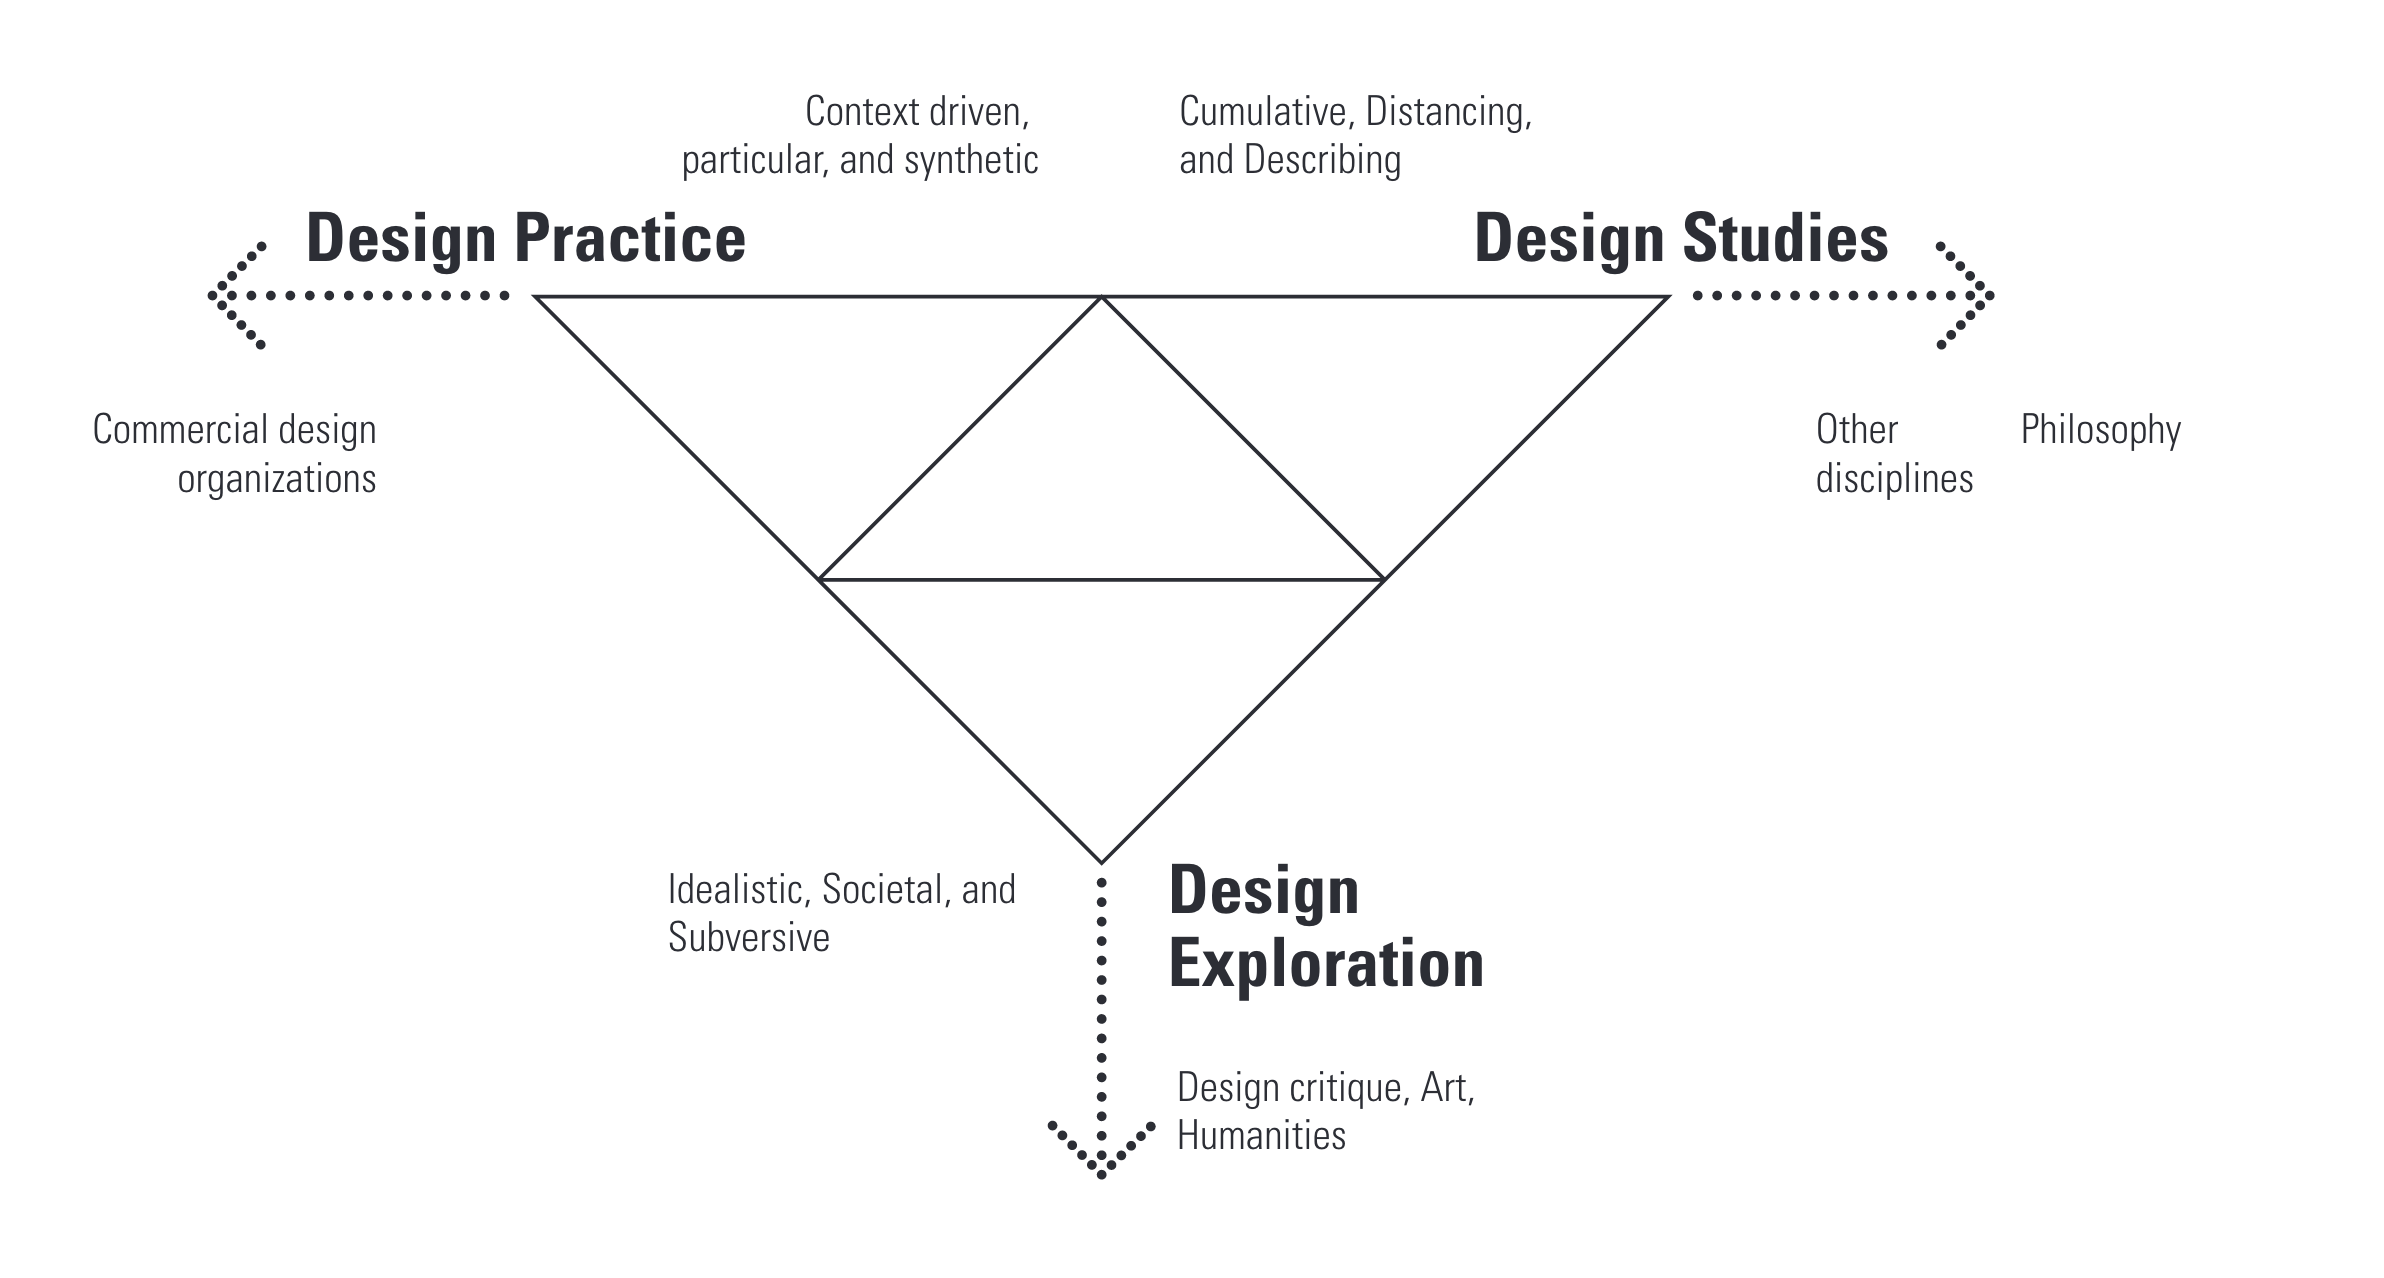
\includegraphics[width=13cm]{pictures/process/triangle.png}
\caption{"The model of interaction design research in its most basic form."}
\autocite[p. 5]{fallman_triangle_2008}
\centering 
\end{figure}

% In terms of doing research through design as a method for interaction design, Zimmerman et. al, explains that what is unique to research though design as an approach, is that it sees the design artefacts as outcomes that can transform the world from its current state to preferred state, which aligns with the domain problems I have accounted for in section 2.0, to address sustainability issues for a more sustainable future. Zimmermann et. al. further explain how the artefacts produced in this type of research become design examples, providing an appropriate channel for research findings to easily transfer to the HCI research and practise communities(Zimmermann et. al, p. 1, 2007).


Design study entails making space for reflections in some kind of structured way on one’s activities: organising reading circles and seminars; and opening up arenas for theoretical, methodological, and philosophical discussions to take place \autocite[p. 18]{fallman_triangle_2008}. The way I have gone forward with this, is to read up on museum practise as evident in chapter 1: Museums, as well as on the topic of sustainability, linking the museum practise up against sustainability. Specifically looking at how sustainability represents a contemporary discourse, and discussing this in relation to how museums want to address and disseminate more contemporary issues to stay relevant. 

+ Design exploration
+ Design Practise


